\documentclass[a4paper]{article}

\usepackage{INTERSPEECH2021}
\usepackage{subfiles}
\usepackage{datatool}
\DTLloaddb{mydata}{scripts/dynamic_latex.csv}

\newcommand{\livedata}[2]{%
    \DTLfetch{#1}{Statistic}{#2}{Value}%
}

\title{Measuring music and prosody: accounting for variation in non-native speech discrimination with L1, L2, music skills, and working memory}
%Paper submission must be anonymous. Only fill in author information for the final PDF.
\name{Author Anonymous$^1$, 
Co-author Anonymous$^1$,
Co-author Anonymous$^1$,
Co-author Anonymous$^1$}
%The maximum number of authors in the author list is twenty. If the number of contributing authors is more than twenty, they should be listed in a footnote or in acknowledgement section, as appropriate.
\address{
  $^1$Author Affiliation}
\email{author@university.edu, 
coauthor@company.com}

\begin{document}

\maketitle
% 
\begin{abstract}
The dynamics of non-native speech perception remain poorly understood, especially in accounting for specialized skills/training. One such skill, musical ability, has been shown to positively impact sensitivity to speech sounds, yet how musical ability is operationalized and measured varies from study to study. Individuals’ musical abilities vary in exposure-duration, skill type (e.g., voice, percussion), and skill-level. Here, we take an individual differences (n=38) approach to explore sensitivity in non-native speech discrimination of prosodic contrasts. We measure language background, general cognitive measures, and three measures of musical ability: auditory-motor temporal integration \cite{Kachlicka_Saito_Tierney_2019}, auditory discrimination \cite[MET;]{Wallentin_Nielsen_Friis-Olivarius_Vuust_Vuust_2010}), and musical sophistication \cite[Gold-MSI;]{Müllensiefen_Gingras_Musil_Stewart_2014}. We measured prosodic sensitivity using three AX discrimination tasks and signal detection measures (d'/c): Mandarin tone (primarily cued by pitch), Italian and Japanese (non-)geminates (primarily cued by duration). Results suggest music background, discrimination, and auditory-motor temporal integration capture related –yet divergent– aspects of music experience. Additionally, music sub-skills (e.g., pitch perception) have unequal contributions to non-native speech sensitivity across languages' respective linguistic cues (e.g., tone). Findings support models of non-native speech perception, which consider cognitive factors and auditory experience outside of language experience.

\end{abstract}
\noindent\textbf{Index Terms}:  Individual differences, Music, Non-native speech perception, Measuring prosody


\section{Introduction}
awesome text

This is how many participants we started with:
\livedata{mydata}{starting_participants}

This is how many participants we ended with:
\livedata{mydata}{kept_participants}

This is how many participants we removed:
\livedata{mydata}{removed_participants}

\section{Outline}
\subfile{outline.tex}

\section{methods}

\subsubsection{participants}

Recruitment of 53 participants for the experiment was
managed through Prolific (Palan & Schitter, 2018) and linked to Gorilla. Not included
in those 60, 37 participants were rejected from participation based on not meeting
initial requirements; including: eight headphone check failures (Milne et al., 2021), 23
eye-calibration failures, five timeouts (90-minute limit), one IRB non-consent. Of the 60
participants who participated in the study, one was removed due to age, two were
removed for other language experiences, three were removed for low accuracy scores
(below three standard deviations of the mean inaccuracies), and five were removed for
having a low frame rate (< 5Hz). As in Porretta et al. (2020), participants were asked
to estimate their total lifetime experience interacting with accented Chinese speakers
(as a percentage of their lifetime interactions). The resulting 49 participants’ reported
amount of Chinese accent experience (range= 0-100 M = 10.47% (SD = 14.13), was
right skewed. Following Porretta et al. (2020), log transformation (with a constant of 1)
and a prior scaling to 0-30 range was employed (range = 0-3.43, M = 0.99, SD = 0.92).

\subsection{Figures}

stuff here Figure~\ref{fig:raw_data}.

\begin{figure}[t]
  \centering
  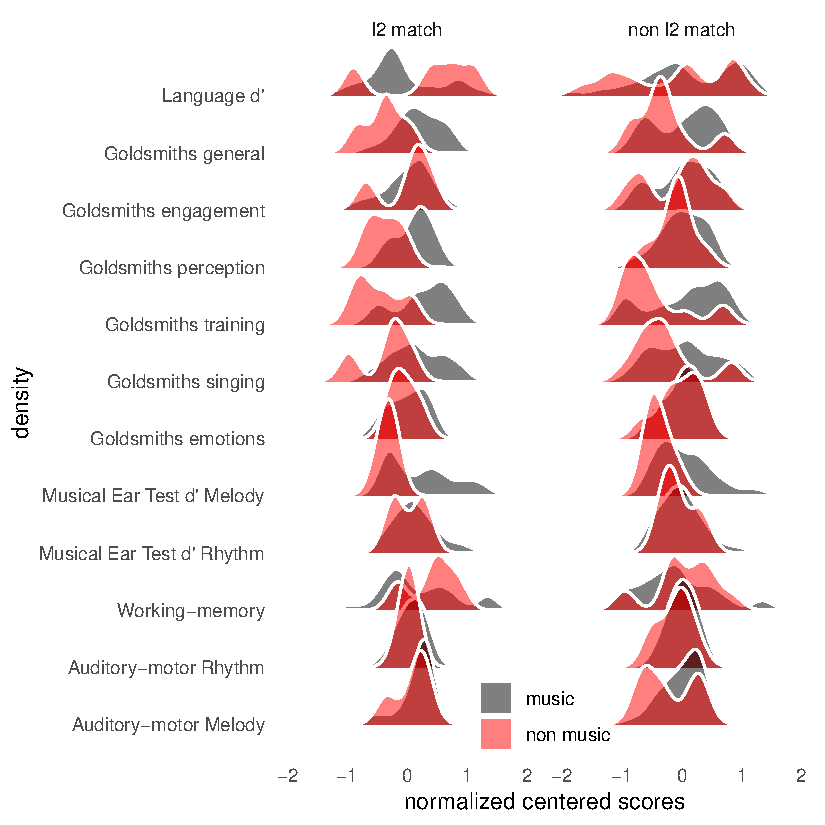
\includegraphics[width=\linewidth]{SP_24_visuals/Normalized_score_distrubutions_by_task.pdf}
  \caption{Raw data}
  \label{fig:raw_data}
\end{figure}

\subsection{Results}

all of our fancy results

~\ref{fig:model}.

\begin{figure}[t]
  \centering
  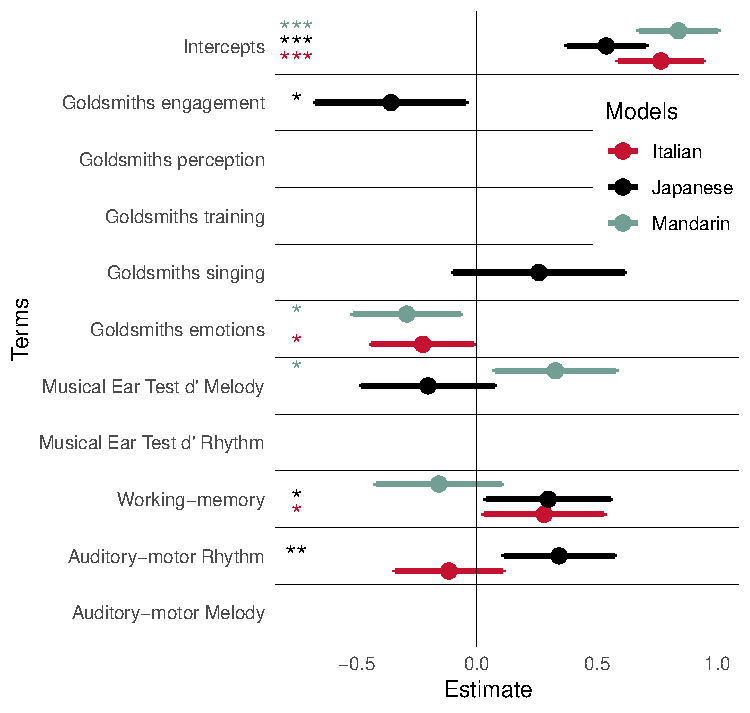
\includegraphics[width=\linewidth]{SP_24_visuals/Japanese,Italian,_Mandarin_max_models_structure:_parsimonious_effects.pdf}
  \caption{model output}
  \label{fig:model}
\end{figure}

\section{Discussion}

\section{Conclusions}

Complex measurement stuff. But, still many things to discover

\section{Acknowledgements}

We would like to thank XXXX and XXXX for funding this project. \\

\bibliographystyle{IEEEtran}

\bibliography{my_references.bib}

\end{document}
